% -*- TeX-master: "main"; fill-column: 72 -*-

\section{Proposal: Encoding Gene Protein Associations in XML}
\label{apdx-gene_association}

This specification drafted by \emph{Brett G. Olivier} and \emph{Frank T. Bergmann} (2013) on behalf of and with contributions by members of the \emph{FBC working group} as well as \emph{FBC} and \emph{SBML} communities.

\subsection{ Introduction and motivation }
\label{intro-ga}

Genome scale reconstructions (GSR) are widely used for biotechnological purposes for example creating or increasing the yield of a specific product, rerouting metabolic pathways and increasing biomass yield on specific substrates. In order to facilitate this GSR's are currently annotated with gene-protein relationships which relates particular genes (implicitly the gene product) with a protein (typically an enzyme or transporter) that carries a specific metabolic flux. In this way it is possible to perform `in silico' gene knockout experiments or otherwise relate particular fluxes to measured gene expression levels.

The problem that this proposal seeks to address is that currently there is no standard way of encoding these gene-protein relationships in an unambiguous and interoperable way. In SBML encoded GSR models these annotations are typically stored as \Notes in a \Reaction.
%
\exampleFile{examples/ex_ga_bigg.txt}
% <p>GENE_ASSOCIATION: CAC1001|CAC1369|CAC1819|CAC2832|CAC3031</p> doesn't encode properly with mikes stylesheet but a classic nonetheless.

Note that each of these annotations was taken from a different model and uses a slightly different syntax either in the `key' or the `value' (bracketing, syntax, attribute definition, etc.). Currently there is no way in \sbmlthreecore or the \FBCPackage to encode model properties embedded in boolean expressions -- a situation this proposal seeks to address.

\pagebreak
\subsection{Proposed syntax and semantics}
\label{syntax-ga}

\begin{figure}[h!]
  \centering
  % Requires \usepackage{graphicx}
  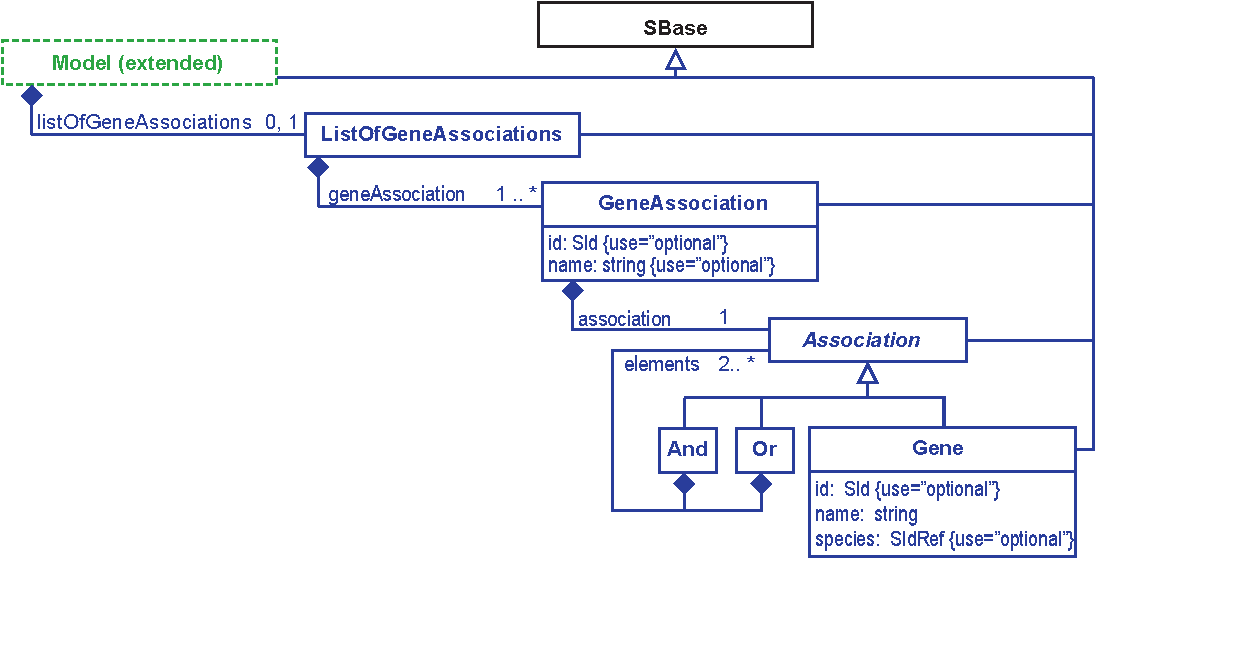
\includegraphics[width=\textwidth]{images/fbc_uml_ga_all.pdf}\\
  \caption{A UML representation of the \FBCPackage. Derived from \SBase, the \FBC classes inherit support for constructs such as SBML \Notes and \Annotation's. See \ref{conventions} for conventions related to this figure. The individual classes are further discussed in the text.}
  \label{fig:fbc_uml_ga_all}
\end{figure}

\subsection{The extended \class{Model} class}
\label{listofgeneassociations-class}


\subsubsection{The \FBC \class{listOfGeneAssociations}}

The \ListOfGeneAssociations extends \sbmlthreecore, is derived from \SBase and inherits the attributes \token{metaid} and \token{sboTerm} as well as the subcomponents for \Annotation and \Notes (as shown in \ref{fig:fbc_uml_ga_all}). If defined \ListOfGeneAssociations must contain at least one \GeneAssociation (as defined below in \ref{geneassociation-class}).

\subsection{The extended \class{Species} class}
\label{species-class-ga}

The \FBCPackage \textsf{Gene Association Proposal} (this document) extends the \sbmlthreecore \Species class (in addition to \token{charge} and \token{chemicalFormula}) with the addition of an attribute \token{isGene}.
%
\begin{figure}[h!]
  \centering
  % Requires \usepackage{graphicx}
  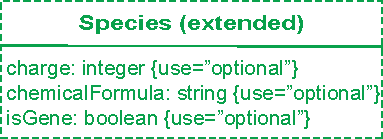
\includegraphics[width=6cm]{images/fbc_uml_species-v2.pdf}\\
  \caption{A UML representation of the extended \SBML \Species class used in
  the \FBCPackage. See \ref{conventions} for conventions related to this
  figure.}
  \label{fig:fbc_uml_species_ga}
\end{figure}

\paragraph{The \token{isGene} attribute}
The optional attribute \token{isGene} contains a \primtype{boolean} referring to the fact that the \Species is not a metabolite that should be included in the reaction network and but rather represents a \Gene product that participates in an \Association. If present, a \Species that has \verb+isGene="true"+ should have at least one \Gene that refers to it via its \token{species} attribute (for more details see \ref{gene-class}).
%
\exampleFile{examples/ex_spec_l3_v2.txt}

\subsection{The \FBC \class{GeneAssociation} class}
\label{geneassociation-class}

The \FBCPackage defines a \GeneAssociation class that derives from \SBase and inherits the attributes \token{metaid} and \token{sboTerm}, as well as the subcomponents for \Annotation and \Notes. As shown in Fig.~ \ref{fig:fbc_uml_ga_all} the \GeneAssociation class connects a \Reaction (flux) with one or more gene (or gene products) in some form of association.

\paragraph{The \token{id} attribute}
The \GeneAssociation class defines an optional attribute: \token{id} of type \primtype{SId}

\paragraph{The \token{reaction} attribute}
The required \token{reaction} attribute of type \primtype{SIdRef}. This attribute must refer to a \Reaction element defined within the enclosing model.

\paragraph{The \token{association} element}
Each \GeneAssociation must contain a single \Association, however, as described in \ref{association-class} an \Association is an abstract class such that \token{association} should contain an instance of one of its sub-classes \GeneAnd, \GeneOr or \Gene.

\begin{figure}[h!]
  \centering
  % Requires \usepackage{graphicx}
  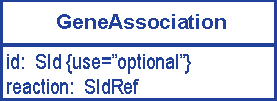
\includegraphics[width=5cm]{images/fbc_uml_ga.pdf}\\
  \caption{A UML representation of the \FBCPackage \GeneAssociation class. See  \ref{conventions} for conventions related to this figure.}
  \label{fig:fbc_uml_ga}
\end{figure}

\paragraph{Encoding the \GeneAssociation}
As described in \ref{geneassociation-class} the \GeneAssociation is simply a container that relates a \Reaction to one of three types of \Association, either holding a single \Gene or two or more genes in an \GeneAnd or \GeneOr relationship. For example the following typical gene--protein association
%
\begin{verbatim}
 ((B3670 and B3671) or (B0077 and B0078) or (B3768 and B3769 and B3767))
\end{verbatim}
%
from the BiGG database \emph{E.~coli} reconstruction (iJR904) \cite{ijr904, bigg} is now encoded in XML as:
%
\exampleFile{examples/spec-example1-ga.txt}


\subsection{The \FBC \class{Association} class}
\label{association-class}

The \FBCPackage defines an abstract \Association class that is derived from \SBase and inherits the attributes \token{metaid} and \token{sboTerm}, as well as the subcomponents for \Annotation and \Notes. It represents either a single gene or a collection of genes and should only ever be instantiated as one of its subclasses: \Gene (\ref{gene-class}), \GeneAnd (\ref{and-class}) and \GeneOr (\ref{or-class}).

\begin{figure}[h!]
  \centering
  % Requires \usepackage{graphicx}
  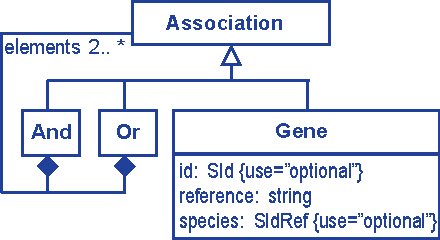
\includegraphics[width=10cm]{images/fbc_uml_ass.pdf}\\
  \caption{A UML representation of the \FBCPackage \Association and derived classes. See \ref{conventions} for conventions related to this figure.}
  \label{fig:fbc_uml_ass}
\end{figure}

\subsection{The \FBC \class{Gene} class}
\label{gene-class}

The \FBCPackage defines a \Gene class that represents a gene (or gene product) is derived from an \Association and thereby inherits the \SBase attributes \token{metaid} and \token{sboTerm}, as well as the subcomponents for \Annotation and \Notes as described in \ref{fig:fbc_uml_ass}.

It is highly recommended that for future interoperability genes should be annotated using MIRIAM compliant mechanisms available via the SBML \Annotation mechanism.

\paragraph{The \token{id} attribute}
The \GeneAssociation class defines an optional attribute \token{id} of type \primtype{SId}.

\paragraph{The \token{species} attribute}
The optional attribute \token{species} attribute of type \primtype{SIdRef} can  refer to a \Species element defined within the enclosing model. The intention here is to allow gene--protein associations to be linked to \Species which may represent them in the model thus bridging two conceptually different (yet equally valid) ways of representing such relations. This attribute should be used in conjunction with the extended \Species attribute \token{isGene} (see \ref{species-class-ga} for details).

\paragraph{The \token{reference} attribute}
The reference attribute

\exampleFile{examples/spec-example1-gene.txt}


\subsection{The \FBC \class{And} class}
\label{and-class}

The \FBCPackage defines an \GeneAnd class that represents a gene (or gene product) and is derived from and \Association and thereby inherits the \SBase attributes \token{metaid} and \token{sboTerm}, as well as the subcomponents for \Annotation and \Notes as described in \ref{fig:fbc_uml_ass}. This class represents a set of two or more associations that are related in an order independent \emph{`and'} relationship.

\paragraph{The \token{elements} element}
Each \GeneAnd must contain two or more instances (not necessarily of the same type) of any \Association subclass (\GeneAnd, \GeneOr, \Gene).

\exampleFile{examples/spec-example1-geneand.txt}

\subsection{The \FBC \class{Or} class}
\label{or-class}

The \FBCPackage defines an \GeneOr class that represents a gene (or gene product) and is derived from and \Association and thereby inherits the \SBase attributes \token{metaid} and \token{sboTerm}, as well as the subcomponents for \Annotation and \Notes as described in \ref{fig:fbc_uml_ass}. This class represents a set of two or more associations that are related in an order independent \emph{`or'} relationship.

\paragraph{The \token{elements} element}
Each \GeneOr must contain two or more instances (not necessarily of the same type) of any \Association subclass (\GeneAnd, \GeneOr, \Gene).

\exampleFile{examples/spec-example1-geneor.txt}
